\documentclass[runningheads,a4paper]{llncs}
%
\usepackage{natbib} % bibliography stuff
%
\usepackage{graphicx} % allows for working with images
\DeclareGraphicsExtensions{.pdf,.png,.jpeg,.jpg} % configures latex to look for the following image extensions
%
\usepackage{setspace} % allows for configuring the linespacing in the document
%\singlespacing
\onehalfspacing
%\doublespacing
%
\usepackage{amsmath}
%
\usepackage{appendix}
%
\usepackage{multirow}
%
\usepackage{booktabs,array,dcolumn}
%
\usepackage{float}
%
\usepackage{eurosym}
%
\usepackage{caption}
\captionsetup[table]{skip=10pt}
\captionsetup{compatibility=false}
\usepackage{subcaption}
%
\usepackage[toc]{glossaries}
\makeglossaries
%
\usepackage{amssymb}
\setcounter{tocdepth}{4}
%
\usepackage{url}
\urldef{\mailsa}\path|dkirwan@tssg.org, someone@somewhere.com, another@abc.com|
\newcommand{\keywords}[1]{\par\addvspace\baselineskip
\noindent\keywordname\enspace\ignorespaces#1}

%Optional Package to add PDF bookmarks and hypertext links
\usepackage[pdftex,hypertexnames=false,linktocpage=true]{hyperref}
\hypersetup{colorlinks=true,linkcolor=black,anchorcolor=black,citecolor=black,filecolor=black,urlcolor=black,bookmarksnumbered=true,pdfview=FitB}

\begin{document}
\mainmatter  % start of an individual contribution

% first the title is needed
\title{An Introduction to Arduino \\a low cost digital prototyping platform}

% a short form should be given in case it is too long for the running head
\titlerunning{Introduction to Arduino}
%

% the name(s) of the author(s) follow(s) next
%
% Chinese authors should write their first names(s) in front of
% their surnames. This ensures that the names appear correctly in
% the running heads and the author index.
%
\author{David Kirwan%
%\thanks{Please note that the LNCS Editorial assumes that all authors have used
%the western naming convention, with given names preceding surnames. This determines
%the structure of the names in the running heads and the author index.}%
\and Someone Else \and An Other}
%
\authorrunning{Observing Jovian Decametric Radio Emissions}
% (feature abused for this document to repeat the title also on left hand pages)

% the affiliations are given next; don't give your e-mail address
% unless you accept that it will be published
\institute{South East Makerspace\\Old Printworks, Thomas Hill\\Waterford City, X91 TW63\\
\mailsa\\
\url{https://www.southeastmakerspace.org}}
%

%
% a more complex sample for affiliations and the mapping to the
% corresponding authors can be found in the file "llncs.dem"
% (search for the string "\mainmatter" where a contribution starts).
% "llncs.dem" accompanies the document class "llncs.cls".
%
%\toctitle{Thesis Proposal}
\tocauthor{SEMS}
\maketitle

%
\begin{abstract}
\begin{figure}
	\centering
	
\includegraphics[width=8cm]{images/sems}
\end{figure}
What is an Arduino? Some information about what this workshop hopes to achieve etc. Lorem ipsum dolor sit amet, consectetur adipiscing elit. Aenean imperdiet congue nisi, eu ultrices elit sollicitudin nec. Vestibulum vitae pretium enim. Mauris eu nulla lectus. Donec eu arcu sem. Pellentesque quis metus eget quam efficitur fringilla tristique vitae neque. Nulla at erat ac felis mollis vulputate id vitae justo. Donec ac rutrum neque. Pellentesque at mollis arcu, quis blandit orci. Cum sociis natoque penatibus et magnis dis parturient montes, nascetur ridiculus mus.
\keywords{arduino, digital electronics, prototyping, introduction}
\end{abstract}
%

%% Acknowledgements
\newpage
\chapter*{Acknowledgements}
<<<<<<< HEAD
I'd like to thank my legs, for always supporting me; my arms, who are always by my side and lastly my fingers, I can always count on them.
=======
I'd like to thank my legs, for always supporting me; my arms, who are always by my side and lastly my fingers, I can always count on them.
>>>>>>> 4d7d12c... - minor changes

<<<<<<< HEAD
=======
%\newpage
%\chapter*{Acknowledgements}
<<<<<<< HEAD
I'd like to thank my legs, for always supporting me; my arms, who are always by my side and lastly my fingers, I can always count on them.
=======
I'd like to thank my legs, for always supporting me; my arms, who are always by my side and lastly my fingers, I can always count on them.
>>>>>>> 4d7d12c... - minor changes

=======
>>>>>>> 4d7d12c... - minor changes
%

%
\tableofcontents
%

%
\newpage
\listoffigures
\addcontentsline{toc}{chapter}{List of Figures}
%

%
\newpage
\listoftables
\addcontentsline{toc}{chapter}{List of Tables}

%%%%%%%%%%%%%%%%%%%%%%%%%%%%%%%%%%%%%%%%%%%%%%%%%%%%%%%%%%%%%%%%%%%%%%%%%%%%%%%%%%%%%
%

%
\newpage
\chapter*{Introduction}
\addcontentsline{toc}{chapter}{Introduction}

\section*{asdf}
\addcontentsline{toc}{section}{asdf}

asdf

\chapter*{Experiment 1}
\addcontentsline{toc}{chapter}{Experiment 1}

Outline each experiment in a separate chapter
\chapter*{Experiment 2 - Button}
\addcontentsline{toc}{chapter}{Experiment 2 - Button}
We wire up the experiment as shown in the diagram fig:~\ref{fig:exp2_button}. And upload the sketch code in the next section on page:~\pageref{sketch:exp2}.

%
\begin{figure}[ht]
	\centering
	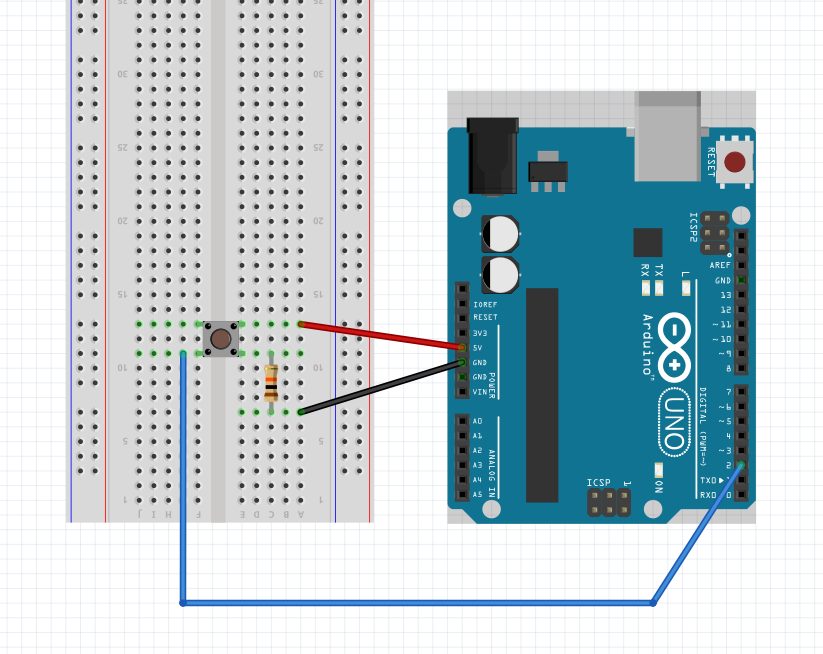
\includegraphics[width=12cm]{images/08}
	\caption{Button activated LED \citep{fritzing-15}}
	\label{fig:exp2_button}
\end{figure}
%

The LED will light up when the button is pressed.

\newpage
\section*{Sketch Code}
\label{sketch:exp2}
\begin{lstlisting}
/*
Button activated LED

This example code is in the public domain.
*/

 
// Pin 13 has an LED connected on most Arduino boards.
// give it a name:
int led = 13;

// the setup routine runs once when you press reset:
void setup() {                
  // initialize the digital pin as an output.
  pinMode(led, OUTPUT);     
}

// the loop routine runs over and over again forever:
void loop() {
  digitalWrite(led, HIGH);   // turn the LED on (HIGH is the voltage level)
}

\end{lstlisting}
\chapter*{Experiment 3 - Generating Music}
\addcontentsline{toc}{chapter}{Experiment 3 - Generating Music}
We wire up the experiment as shown in the diagram fig:~\ref{fig:exp3_music}. And upload the sketch code in the next section on page:~\pageref{sketch:exp3}.

%
\begin{figure}[ht]
	\centering
	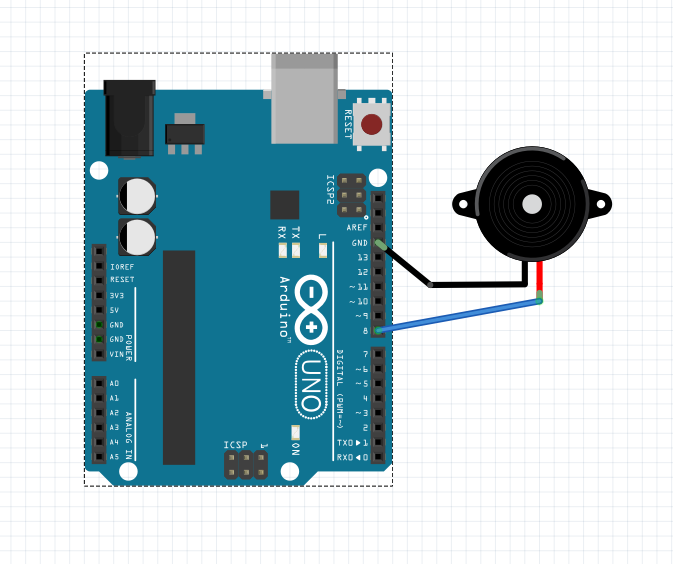
\includegraphics[width=12cm]{images/09}
	\caption{Play musical notes through a speaker \citep{fritzing-15}}
	\label{fig:exp3_music}
\end{figure}
%

As soon as the \gls{Arduino} boots it should play a series of musical notes and then stop. For more information see the online reference page for the functions used in this experiment here: https://www.arduino.cc/en/Reference/Tone

\newpage
\section*{Sketch Code}
\label{sketch:exp3}
\begin{lstlisting}
/*
Melody - Plays a melody
This example code is in the public domain.
*/
#include "pitches.h"

int melody[] = { // notes in the melody:
  NOTE_C4, NOTE_G3, NOTE_G3, NOTE_A3, NOTE_G3, 0, NOTE_B3, NOTE_C4
};

// note durations: 4 = quarter note, 8 = eighth note, etc.:
int noteDurations[] = {
  4, 8, 8, 4, 4, 4, 4, 4
};

void setup() {
  // iterate over the notes of the melody:
  for (int thisNote = 0; thisNote < 8; thisNote++) {
    // to calculate the note duration, take one second
    // divided by the note type.
    //e.g. quarter note = 1000 / 4, eighth note = 1000/8, etc.
    int noteDuration = 1000 / noteDurations[thisNote];
    tone(8, melody[thisNote], noteDuration);
    // to distinguish the notes, set a minimum time between them.
    // the note's duration + 30% seems to work well:
    int pauseBetweenNotes = noteDuration * 1.30;
    delay(pauseBetweenNotes);
    noTone(8);
  }
}

void loop() {
  // no need to repeat the melody.
}

// ********************* pitches.h ************************

/*************************************************
* Public Constants
*************************************************/

#define NOTE_B0  31
#define NOTE_C1  33
#define NOTE_CS1 35
#define NOTE_D1  37
#define NOTE_DS1 39
#define NOTE_E1  41
#define NOTE_F1  44
#define NOTE_FS1 46
#define NOTE_G1  49
#define NOTE_GS1 52
#define NOTE_A1  55
#define NOTE_AS1 58
#define NOTE_B1  62
#define NOTE_C2  65
#define NOTE_CS2 69
#define NOTE_D2  73
#define NOTE_DS2 78
#define NOTE_E2  82
#define NOTE_F2  87
#define NOTE_FS2 93
#define NOTE_G2  98
#define NOTE_GS2 104
#define NOTE_A2  110
#define NOTE_AS2 117
#define NOTE_B2  123
#define NOTE_C3  131
#define NOTE_CS3 139
#define NOTE_D3  147
#define NOTE_DS3 156
#define NOTE_E3  165
#define NOTE_F3  175
#define NOTE_FS3 185
#define NOTE_G3  196
#define NOTE_GS3 208
#define NOTE_A3  220
#define NOTE_AS3 233
#define NOTE_B3  247
#define NOTE_C4  262
#define NOTE_CS4 277
#define NOTE_D4  294
#define NOTE_DS4 311
#define NOTE_E4  330
#define NOTE_F4  349
#define NOTE_FS4 370
#define NOTE_G4  392
#define NOTE_GS4 415
#define NOTE_A4  440
#define NOTE_AS4 466
#define NOTE_B4  494
#define NOTE_C5  523
#define NOTE_CS5 554
#define NOTE_D5  587
#define NOTE_DS5 622
#define NOTE_E5  659
#define NOTE_F5  698
#define NOTE_FS5 740
#define NOTE_G5  784
#define NOTE_GS5 831
#define NOTE_A5  880
#define NOTE_AS5 932
#define NOTE_B5  988
#define NOTE_C6  1047
#define NOTE_CS6 1109
#define NOTE_D6  1175
#define NOTE_DS6 1245
#define NOTE_E6  1319
#define NOTE_F6  1397
#define NOTE_FS6 1480
#define NOTE_G6  1568
#define NOTE_GS6 1661
#define NOTE_A6  1760
#define NOTE_AS6 1865
#define NOTE_B6  1976
#define NOTE_C7  2093
#define NOTE_CS7 2217
#define NOTE_D7  2349
#define NOTE_DS7 2489
#define NOTE_E7  2637
#define NOTE_F7  2794
#define NOTE_FS7 2960
#define NOTE_G7  3136
#define NOTE_GS7 3322
#define NOTE_A7  3520
#define NOTE_AS7 3729
#define NOTE_B7  3951
#define NOTE_C8  4186
#define NOTE_CS8 4435
#define NOTE_D8  4699
#define NOTE_DS8 4978
\end{lstlisting}
\chapter*{asdf}
\addcontentsline{toc}{chapter}{asdf}
asdf
\chapter*{Experiment 5 - Phenakistoscope Creation}
\addcontentsline{toc}{chapter}{Experiment 5 - Phenakistoscope Creation}

Outline each experiment in a separate chapter

\citep{kalif-15-a} \citep{kalif-15-b}
\newpage
\chapter*{Conclusions}
\addcontentsline{toc}{chapter}{Conclusions}

\begin{itemize}
  \item sum up the answers to all the questions
  \item state contributions again
  \item where my work fits in the grander scheme
  \item further work
\end{itemize}

\section*{Final Summary}
\addcontentsline{toc}{section}{Final Summary}

In conclusion while this research was necessarily limited by the available time and resources, never the less a contribution to new knowledge was made through the development of supporting open source tools and resources which might enable further research in this field in the future. There are many opportunities with several existing large radio telescope arrays, such as the Atacama Large Millimetre/submillimetre Array (ALMA) and the Low Frequency Array (LOFAR), while others are in the early planning stages and are due to be built in the near future like the Square Kilometre Array (SKA). I am encouraged to continue working on this and similar topics and I am currently considering applying to a doctoral program which might allow the pursuit of a research career in astronomy.
%

%
%%%%%%%%%%%%%%%%%%%%%%%%%%%%%%%%%%%%%%%%%%%%%%%%%%%%%%%%%%%%%%%%%%%%%%%%%%%%%%%%%%%%%
%
%
\newglossaryentry{Arduino}
{
  name={Arduino},
  description={an open-source electronics platform based on easy-to-use hardware and software. It's intended for anyone making interactive projects. https://www.arduino.cc},
  sort=Arduino
}
%
\renewcommand*{\glsclearpage}{}
\printglossaries
%

%
\appendix
\chapter*{Appendix}
\addcontentsline{toc}{chapter}{Appendices}

<<<<<<< HEAD
=======
%\appendix
%\chapter*{Appendix}
\addcontentsline{toc}{chapter}{Appendices}

=======
>>>>>>> 4d7d12c... - minor changes
%

%
\bibliographystyle{plainnat}
\bibliography{bibliography/bibtex}
\addcontentsline{toc}{chapter}{Bibliography}
%

\end{document}


